\documentclass[11pt]{beamer}
\usetheme{Warsaw}
\usepackage[utf8]{inputenc}
\usepackage[english]{babel}
\usepackage{amsmath}
\usepackage{amsfonts}
\usepackage{amssymb}
\usepackage{graphicx}
\usepackage{listings}
\lstset{ % General setup for the package
	language=bash,
	basicstyle=\small\sffamily,
	numbers=left,
 	numberstyle=\tiny,
	frame=tb,
	tabsize=4,
	columns=fixed,
	showstringspaces=false,
	showtabs=false,
	keepspaces=true,
	breaklines=true,
	moredelim=[is][\color{red}\underbar]{_}{_}
}
\AtBeginSection[]{
  \begin{frame}
  \vfill
  \centering
  \begin{beamercolorbox}[sep=8pt,center,shadow=true,rounded=true]{title}
    \usebeamerfont{title}\insertsectionhead\par%
  \end{beamercolorbox}
  \vfill
  \end{frame}
}
\author{Mathieu Valois - M1 Informatique}
\title{ShockWorm - A shellshock-based worm}
%\setbeamercovered{transparent} 
%\setbeamertemplate{navigation symbols}{} 
\logo{
\includegraphics[scale=0.3]{cc-by-nc-sa.png}  
\includegraphics[scale=0.1]{shellshock.png}  
\includegraphics[scale=0.5]{unicaen_logo_rvb_noir_V2.png}}
\institute{Université de Caen Basse-Normandie} 
%\date{} 
%\subject{} 
\expandafter\def\expandafter\insertshorttitle\expandafter{%
  \insertshorttitle\hfill%
  \insertframenumber\,/\,\inserttotalframenumber}
\begin{document}

\begin{frame}
\titlepage
\end{frame}

\begin{frame}
\tableofcontents
\end{frame}

\section{What the hell are worms ?}
\begin{frame}{What the hell are worms ?}
\begin{itemize}
\item Self-replicating programs
\item Different than viruses : worms don't use host programs, they stand alone
\item Use security holes to move from machine to machine
\item Can be peaceful or aggressive
\item Travel incredibly faster than viruses because they don't need any user interaction
\end{itemize}
\begin{center}

\includegraphics[scale=0.1]{worm.jpeg}
\end{center}
\end{frame}

\section{The point of my project}
\begin{frame}{The point of my project}
\begin{itemize}
\item The goal is to program a worm, possibly one that doesn't already exist, that can replicate over multiple machines
\item I'm free to chose which security hole I would like it to exploit
\item Then inject the worm in a secured bunch of connected computers that are vulnerable (some might not be) for testing 
\end{itemize}
\end{frame}

\section{The vulnerability: ShellShock}
\begin{frame}{The vulnerability: ShellShock}
\noindent
 \parbox[t]{8cm}{
The shellshock is: 
\begin{itemize}
\item A bash vulnerability
\item Introduced in bash code in 1989 (according to the bash main developer, Brian Fox) and discovered in September 2014 (I'll let you guess how long it went undiscovered)
\item Since bash is massively used on all UNIX systems, ShellShock was present on a lot of machines, from servers to embedded devices and even IP cameras
\end{itemize}}
     \hfill
       \raisebox{\dimexpr-\height+\baselineskip}{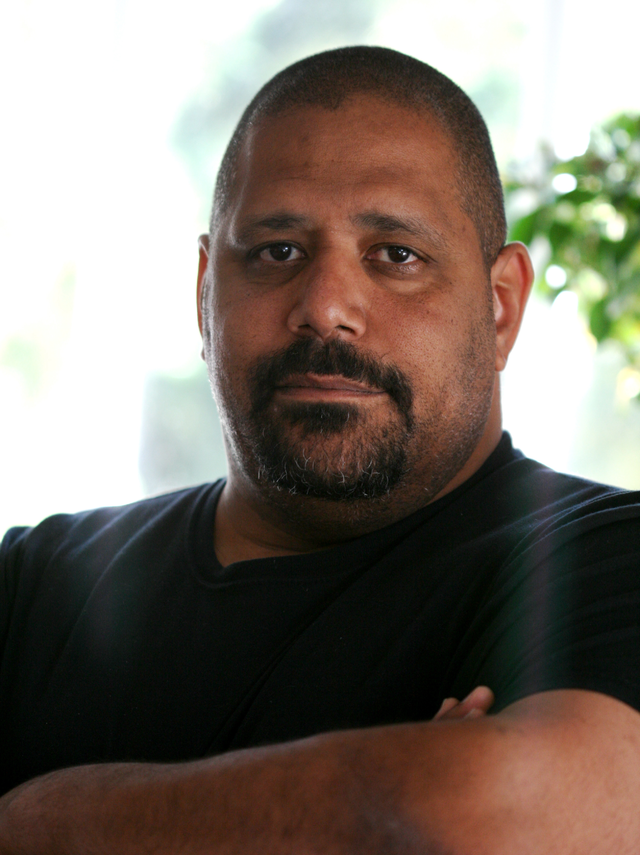
\includegraphics[scale=0.1]{brian_fox.png}}
\end{frame}


\section{What can my worm do ?}
\begin{frame}{What can my worm do ?}

For now, ShellWorm is fitted with these abilities:
\begin{itemize}
\item Moving from an infected (or starting) machine to a new one that is vulnerable (infection)
\item Can be started at boot without root permissions 
\item Can intercept users passwords by overriding the "sudo" command
\end{itemize}


\begin{center}

\includegraphics[scale=0.08]{linux_force.jpg}
\end{center}
\end{frame}

\section{What's next ?}
\begin{frame}{What's next ?}
\begin{itemize}
\item Persist on reboots with root access, to ensure not to be killed or to be able to hide, for example from scanning processes
\item Spy on the system, to get users information and eventually  send it to a remote server
\end{itemize}
\end{frame}

\section{Questions ?}

\begin{frame}{Why did I chose this project ?}
\begin{itemize}
\item I've read interesting books on the subject
\item The moment ShellShock was discovered matched the moment where we had to chose a project
\item No really other interesting E-Secure projects were announced
\end{itemize}
\end{frame}

\end{document}